\documentclass[crop,tikz]{standalone}
\usepackage{amsmath}
\usetikzlibrary{positioning}
\usetikzlibrary{spath3,intersections}


\begin{document}
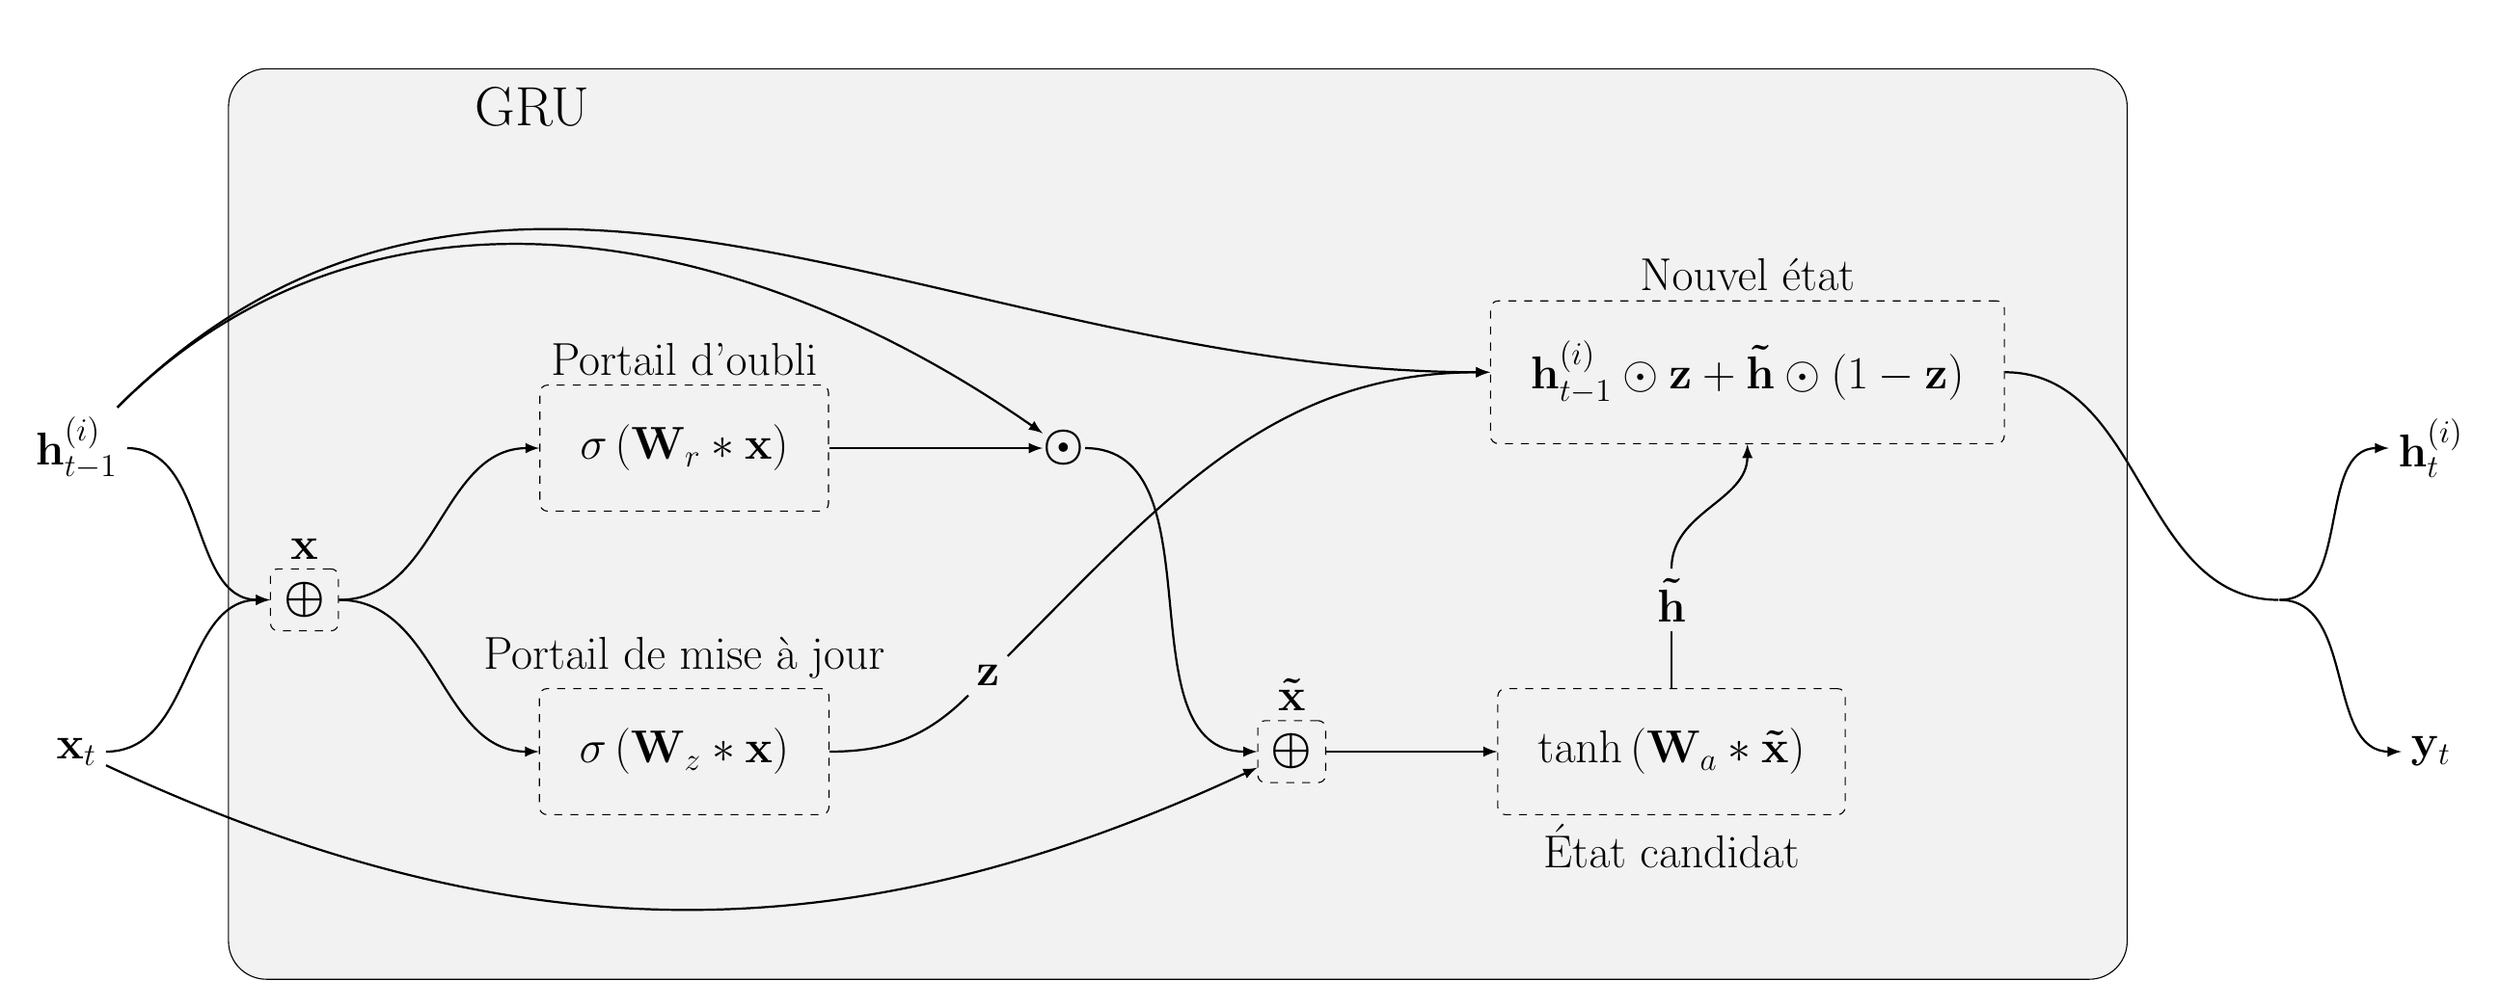
\begin{tikzpicture}[
    node distance=3cm
]
    \draw[rounded corners=0.5cm, fill=black!5, draw=black] (-5, -5) rectangle (20, 7);
    \node (title) at (-1, 6.5) {\huge GRU};
    
    \node (states) at (-7, 2) {\LARGE$\mathbf{h}^{(i)}_{t-1}$};
    \node (x) at (-7, -2) {\LARGE$\mathbf{x}_t$};
    \node[rectangle, rounded corners=0.1cm, dashed, draw=black, label={\LARGE Portail d'oubli}, inner sep=15pt] 
        (reset gate) at (1, 2) {\LARGE $\sigma \left(\mathbf{W}_r \ast \mathbf{x}\right)$};
    \node[rectangle, rounded corners=0.1cm, dashed, draw=black, label={\LARGE Portail de mise à jour}, inner sep=15pt] 
        (update gate) at (1, -2) {\LARGE $\sigma \left(\mathbf{W}_z \ast \mathbf{x}\right)$};
    \node[rectangle, rounded corners=0.1cm, dashed, draw=black, label={\LARGE $\mathbf{x}$}, inner sep=5pt] (concat) at (-4, 0) {\LARGE$\boldsymbol{\oplus}$};
    
    \draw[-latex, thick, in=180, out=0] (states) to (concat);
    \draw[-latex, thick, in=180, out=0] (x) to (concat);
    
    \draw[-latex, thick, in=180, out=0] (concat) to (reset gate);
    \draw[-latex, thick, in=180, out=0] (concat) to (update gate);
    \node[rectangle, rounded corners=0.1cm, dashed, draw=black, label=below:{\LARGE État candidat}, inner sep=15pt] 
        (candidate gate) at (14, -2) {\LARGE $\tanh \left(\mathbf{W}_a \ast \mathbf{\tilde{x}}\right)$};
        
    \node[inner sep=0pt] (multiply) at (6, 2) {\LARGE$\boldsymbol{\odot}$};
    \node[rectangle, rounded corners=0.1cm, dashed, draw=black, label={\LARGE $\mathbf{\tilde{x}}$}, inner sep=5pt] (concat) at (9, -2) {\LARGE$\boldsymbol{\oplus}$};
    
    \draw[-latex, thick] (reset gate) to (multiply);
    \draw[-latex, thick, in=145, out=45] (states) to (multiply);
    
    \draw[-latex, thick, in=205, out=-25] (x) to (concat);
    \draw[-latex, thick, out=0, in=180] (multiply) to (concat);
    \draw[-latex, thick] (concat) to (candidate gate);
    
    \node[rectangle, rounded corners=0.1cm, dashed, draw=black, label={\LARGE Nouvel état}, inner sep=15pt] 
        (new state) at (15, 3) {\LARGE $\mathbf{h}^{(i)}_{t-1} \odot \mathbf{z} + \mathbf{\tilde{h}} \odot (1 - \mathbf{z})$};
        
    \draw[-latex, thick, in=180, out=45] (states) to (new state);
    
    \node%[rectangle, rounded corners=0.1cm, dashed, draw=black, inner sep=5pt] 
        (z) at (5, -1) {\LARGE $\mathbf{z}$};
    \draw[-, thick, out=0, in=225] (update gate) to (z);
    \draw[-latex, thick, out=45, in=180] (z) to (new state);
    
    \node%[rectangle, rounded corners=0.1cm, dashed, draw=black, inner sep=5pt] 
        (htilde) at (14, 0) {\LARGE $\mathbf{\tilde{h}}$};
    \draw[-, thick, out=90, in=270] (candidate gate) to (htilde);
    \draw[-latex, thick, out=90, in=270] (htilde) to (new state);
    
    \node[inner sep=0pt, minimum size=0pt] (div) at (22, 0) {};
    \draw[-, thick, out=0, in=180] (new state) to (div);
    \node (output state) at (24, 2) {\LARGE $\mathbf{h}^{(i)}_{t}$};
    \node (y) at (24, -2) {\LARGE $\mathbf{y}_{t}$};
    \draw[-latex, thick, in=180, out=0] (div) to (output state);
     \draw[-latex, thick, in=180, out=0] (div) to (y);
\end{tikzpicture}
\end{document}
